% VOLUME, SCATTER PLOTS, AND SYSTEMS REVIEW - WORKSHEET 0 (IN-CLASS INSTRUCTION)
\documentclass[12pt, letterpaper, fleqn]{article}

% ----------------------------------------------------------
% PACKAGES
% ----------------------------------------------------------
\usepackage{graphicx}
\usepackage{xcolor}
\usepackage[most]{tcolorbox}
\usepackage{amsmath, amssymb}
\usepackage{fancyhdr}
\usepackage[utf8]{inputenc}
\usepackage[T1]{fontenc}
\usepackage{enumitem}
\usepackage{geometry}
\usepackage{tikz}
\usepackage{needspace}
\usepackage{multicol}

\usetikzlibrary{arrows.meta, calc, positioning, shapes.geometric}

% ----------------------------------------------------------
% PAGE SETUP
% ----------------------------------------------------------
\usepackage{times}
\geometry{letterpaper, top=1.25in, bottom=1.25in, marginpar=0.5in}

% ----------------------------------------------------------
% HEADER / FOOTER
% ----------------------------------------------------------
\newcommand{\logowidth}{3cm}
\setlength{\headheight}{20pt}
\setlength{\footskip}{40pt}

\pagestyle{fancy}
\fancyhf{}
\fancyhead[C]{\small\bfseries Volume, Scatter Plots, and Systems Review}
\fancyfoot[L]{\raisebox{2pt}{
\includegraphics[width=\logowidth]{../kss.png}}}
\fancyfoot[C]{\thepage}
\fancyfoot[R]{8.25.0}

\renewcommand{\footrulewidth}{0.2pt}

% ----------------------------------------------------------
% THEME COLOR
% ----------------------------------------------------------
\definecolor{customteal}{HTML}{2fbdb9}

% ----------------------------------------------------------
% HELPER MACROS
% ----------------------------------------------------------
\newcommand{\blank}{\underline{\hspace{2.2cm}}}
\newcommand{\blanklong}{\underline{\hspace{6.5cm}}}
\newcommand{\blankshorter}{\underline{\hspace{1.5cm}}}

% ----------------------------------------------------------
% DOCUMENT
% ----------------------------------------------------------
\begin{document}

\textbf{Name:} \underline{\hspace{5cm}}
\hfill
\textbf{Date:} \underline{\hspace{3cm}}\\

% ==========================================================
% SECTION 1: FOUNDATION
% ==========================================================
\begin{tcolorbox}[colback=customteal!20]
    \large\textcolor{black}{\textbf{Foundation: Core Concepts Review}}
\end{tcolorbox}

\vspace{3mm}

\noindent
This unit reviews the final three pillars of 8th grade math.

\begin{itemize}
    \item \textbf{Volume:} The space inside a 3D object.
    \begin{itemize}
        \item Cylinder: $V = \pi r^2 h$
        \item Cone: $V = \dfrac{1}{3}\pi r^2 h$
        \item Sphere: $V = \dfrac{4}{3}\pi r^3$
    \end{itemize}
    \item \textbf{Scatter Plots:} Graphing data points to see if there is an association (Positive, Negative, or None). A line of best fit can be drawn to make predictions.
    \item \textbf{Systems of Equations:} Finding where two lines cross. This point $(x,y)$ is the one solution that makes both equations true. You can solve by Graphing, Substitution, or Elimination.
\end{itemize}

\vspace{4mm}

% ==========================================================
% VISUAL REPRESENTATION
% ==========================================================
\begin{tcolorbox}[colback=white, colframe=black!25, boxrule=0.6pt, arc=4mm, left=6mm, right=6mm, top=5mm, bottom=5mm]

\textbf{Visual Representation: Systems of Equations}

\medskip

\begin{center}
\begin{tikzpicture}[scale=0.8]

% System 1 (One Solution)
\begin{scope}[shift={(0,0)}]
\draw[thick,->] (-2,0) -- (3,0);
\draw[thick,->] (0,-2) -- (0,3);
\draw[thick, blue] (-1, -2) -- (2, 3);
\draw[thick, red] (-1, 2) -- (2, -1);
\filldraw[black] (0.8, 1) circle (2.5pt);
\node[below] at (0.5, -2.5) {One Solution};
\end{scope}

% System 2 (No Solution)
\begin{scope}[shift={(5,0)}]
\draw[thick,->] (-2,0) -- (3,0);
\draw[thick,->] (0,-2) -- (0,3);
\draw[thick, blue] (-2, -1) -- (2, 3);
\draw[thick, red] (-1, -2) -- (3, 2);
\node[below] at (0.5, -2.5) {No Solution};
\node[font=\footnotesize] at (0.5, -3) {(Parallel Lines)};
\end{scope}

% System 3 (Infinite Solutions)
\begin{scope}[shift={(10,0)}]
\draw[thick,->] (-2,0) -- (3,0);
\draw[thick,->] (0,-2) -- (0,3);
\draw[line width=2pt, blue] (-2, 2) -- (2, -2);
\draw[dashed, red, thick] (-2, 2) -- (2, -2);
\node[below] at (0.5, -2.5) {Infinite Solutions};
\node[font=\footnotesize] at (0.5, -3) {(Same Line)};
\end{scope}

\end{tikzpicture}
\end{center}

\end{tcolorbox}

\vspace{4mm}

\newpage

% ==========================================================
% WORKED EXAMPLES
% ==========================================================
\begin{tcolorbox}[colback=customteal!20]
\large\textcolor{black}{\textbf{Reviewing Scientific Notation}}
\end{tcolorbox}

\vspace{3mm}

\begin{tcolorbox}[colback=white, colframe=black!25, boxrule=0.6pt, arc=4mm, left=6mm, right=6mm, top=5mm, bottom=5mm]

\textbf{Worked Example 1: Solving a System by Substitution}

\medskip

\textbf{Problem:} Solve: \ \ $y = -3x + 5$ \ \ and \ \ $2x + y = 4$

\medskip

\textbf{Solution:}
\begin{itemize}
    \item \textbf{Step 1:} Substitute $(-3x + 5)$ for $y$ in the second equation.
    \[ 2x + (-3x + 5) = 4 \]
    \item \textbf{Step 2:} Combine like terms.
    \[ -x + 5 = 4 \]
    \item \textbf{Step 3:} Solve for $x$.
    \[ -x = -1 \implies x = 1 \]
    \item \textbf{Step 4:} Plug $x=1$ back into the first equation.
    \[ y = -3(1) + 5 = 2 \]
    \item \textbf{Answer:} The solution is the point $(1, 2)$.
\end{itemize}

\end{tcolorbox}

\vspace{4mm}

% ==========================================================
% PRACTICE 1
% ==========================================================
\begin{tcolorbox}[colback=white!15, colframe=black, boxrule=1.5pt, arc=4mm, left=6mm, right=6mm, top=5mm, bottom=5mm]

\textbf{Guided Practice: Concept Checks}

\medskip

\noindent
\textbf{1.} Find the volume of a sphere with a radius of $3\text{ cm}$. Leave your answer in terms of $\pi$.
\vspace{2cm}

\noindent
\textbf{2.} Does the equation $y = 5x - 2$ represent a positive or negative association if graphed as a trend line?
\vspace{1cm}

\noindent
\textbf{3.} Solve the system by elimination:
\begin{align*}
    x + y &= 10 \\
    x - y &= 2
\end{align*}
\vspace{2cm}

\end{tcolorbox}

\newpage

% ==========================================================
% THINKING PROBLEM
% ==========================================================
\begin{tcolorbox}[colback=customteal!20]
\large\textcolor{black}{\textbf{Deeper Thinking: Pulling It All Together}}
\end{tcolorbox}

\vspace{3mm}

\begin{tcolorbox}[colback=white!15, colframe=black, boxrule=1.5pt, arc=4mm, left=6mm, right=6mm, top=5mm, bottom=5mm]

\textbf{Deeper Thinking Problem 1: The Water Tanks}

\medskip

\noindent
There are two cylindrical water tanks. 

\begin{itemize}
    \item \textbf{Tank A} has a radius of $2\text{ ft}$ and a height of $10\text{ ft}$. It is currently completely full, but water is draining out at a rate of $5\pi\text{ cubic feet per minute}$.
    \item \textbf{Tank B} is identical in size to Tank A. It is currently empty, but water is being pumped in at a rate of $3\pi\text{ cubic feet per minute}$.
\end{itemize}

\vspace{5mm}

\noindent
\textbf{a)} Calculate the total volume of Tank A (in terms of $\pi$). This is its starting amount of water.

\vspace{2cm}

\noindent
\textbf{b)} Write a linear equation representing the volume of water ($y$) in Tank A after $x$ minutes.

\vspace{2cm}

\noindent
\textbf{c)} Write a linear equation representing the volume of water ($y$) in Tank B after $x$ minutes.

\vspace{2cm}

\noindent
\textbf{d)} Set up a system of equations to find out exactly how many minutes it will take for both tanks to have the exact same amount of water. Solve the system.

\vspace{3cm}

\end{tcolorbox}

\end{document}
